\documentclass[a4paper]{article}
\usepackage[english]{babel}
\usepackage[utf8]{inputenc}
\usepackage{graphicx}
\usepackage{enumitem}
\usepackage{blindtext}

\graphicspath{ {./images/} }
\setlength\parindent{0pt}

\title{CS2200 Homework 4}
\author{Evan Wilcox}
\date{Due March 19, 2019}

\begin{document}
  \maketitle

  \begin{enumerate}

    \item Write a Python NDFSA+$\epsilon$ simulator. \\
    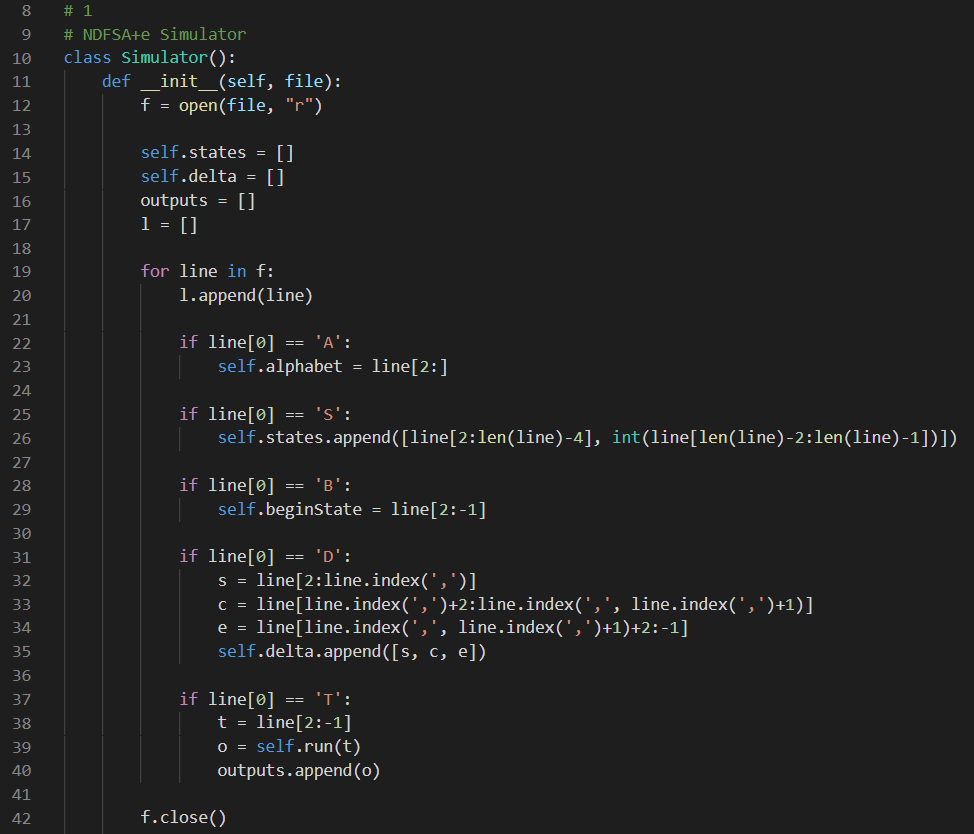
\includegraphics[scale=0.5]{1a} \\
    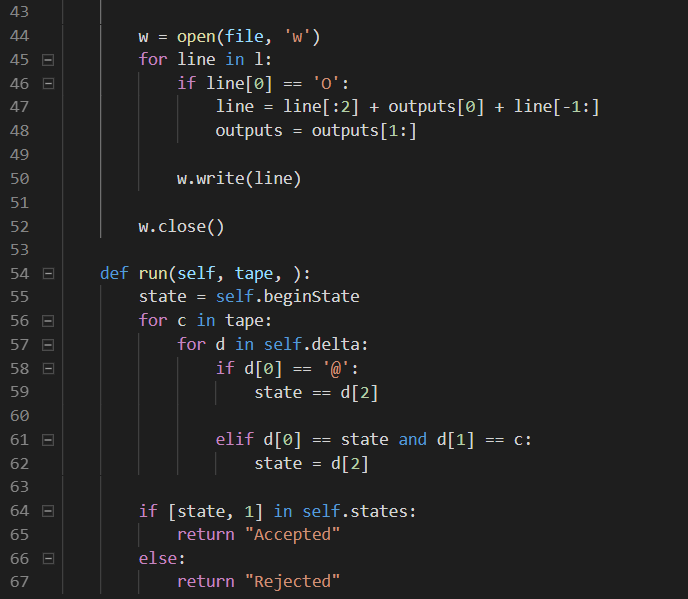
\includegraphics[scale=0.5]{1b}    




    \newpage
    \item Write a program that can generate a Graphviz file from either a .fsa
    or .ndfsa file. \\

    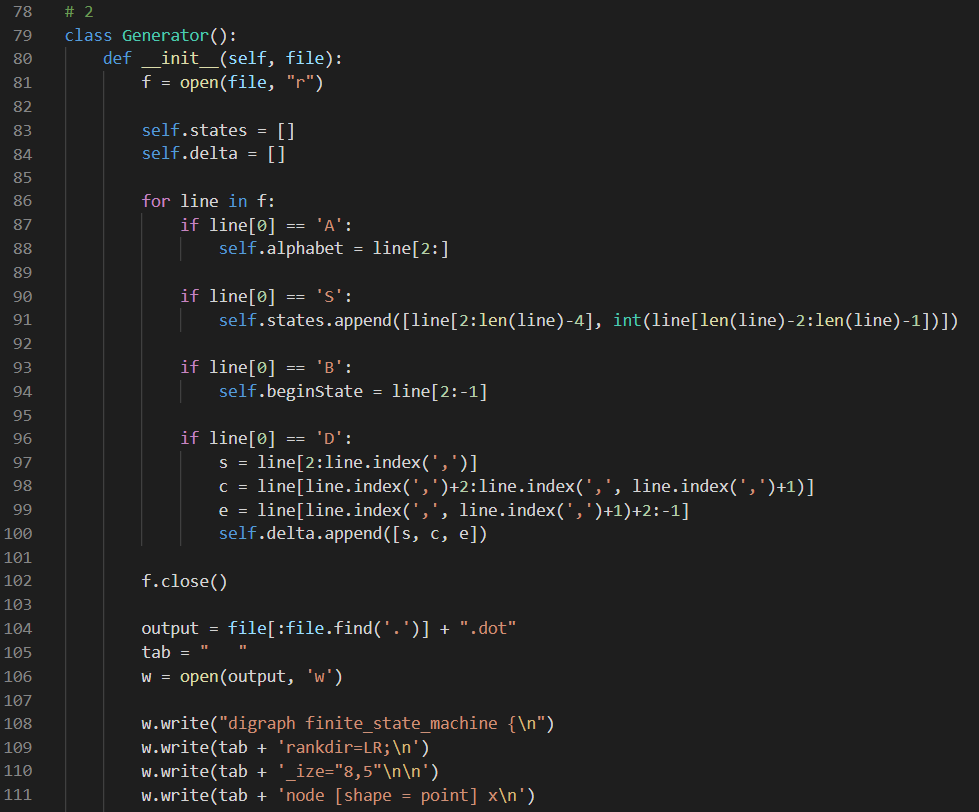
\includegraphics[scale=0.65]{2a} \\ 
    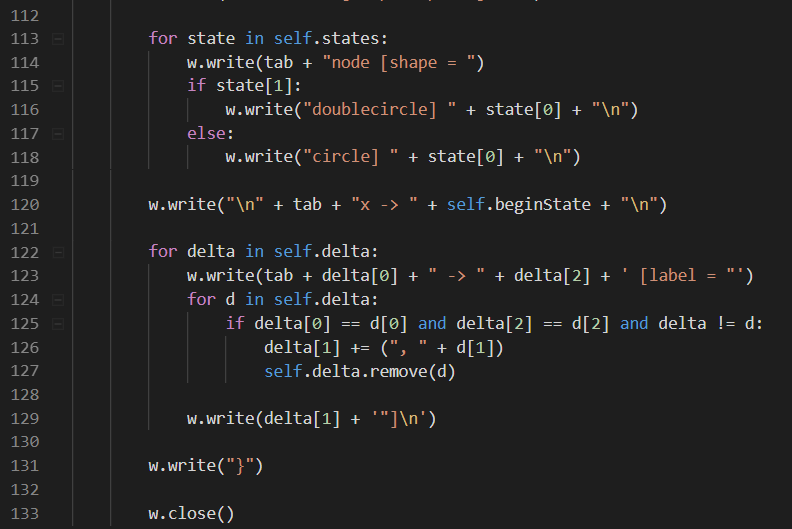
\includegraphics[scale=0.65]{2b} 
    
    

    \addtocounter{enumi}{1}

    \newpage
    \item For each of the following, find a FSA automaton that recognizes the
    language or prove that there is no FSA that recognizes the language.
    
    \begin{enumerate}
    
      \item L$_{1} = \{$ all binary strings divisible by 2 $\}$ \\
      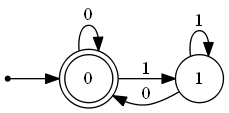
\includegraphics[scale=0.5]{5a}
      \begin{verbatim}
A 01
S 0, 1
S 1, 0
B 0
D 0, 0, 0
D 0, 1, 1
D 1, 0, 0
D 1, 1, 1
T 
O Accepted
T 1
O Rejected
T 0
O Accepted
T 11
O Rejected
T 00
O Accepted
T 10
O Accepted
T 01
O Rejected
T 100101010100
O Accepted
T 0011001101001101
O Rejected
T 111111100000000110
O Accepted 
      \end{verbatim}
    
      \newpage
      \item L$_{2} = \{$ all binary strings divisible by 7 $\}$ \\
      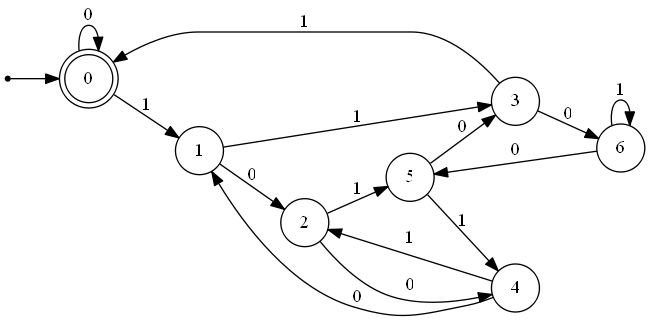
\includegraphics[scale=0.5]{5b}
      \begin{verbatim}
A 01
S 0, 1
S 1, 0
S 2, 0
S 3, 0
S 4, 0
S 5, 0
S 6, 0
B 0
D 0, 0, 0
D 0, 1, 1
D 1, 0, 2
D 1, 1, 3
D 2, 0, 4
D 2, 1, 5
D 3, 0, 6
D 3, 1, 0
D 4, 0, 1
D 4, 1, 2
D 5, 0, 3
D 5, 1, 4
D 6, 0, 5
D 6, 1, 6
T 
O Accepted
T 1
O Rejected
T 0
O Accepted
T 111
O Accepted
T 110
O Rejected
T 1110
O Accepted
T 11101
O Rejected
T 11100
O Accepted
T 0011001101001100
O Accepted
T 111111100000011111
O Accepted 
      \end{verbatim}


      \item L$_{3} = \{$ all unary strings that represent prime numbers $\}$ \\
      
      Let $w = 1^{p}$ where $p$ is a prime number. $w \in$ L$_{3}$. L$_{3}$ can not be 
      represented by a FSA because FSA can only represent regular languages and 
      L$_{3}$ does not produce a regular language. We know this because using the 
      Pumping Lemma, $1^{p}$ can be pumped. \\

      \item L$_{4} = \{$ all unary strings that represent composite numbers $\}$ \\
      
      Let $w = 1^{p}$ where $p$ is a composite number. $w \in$ L$_{3}$. L$_{3}$ can not be 
      represented by a FSA because FSA can only represent regular languages and 
      L$_{3}$ does not produce a regular language. We know this because using the 
      Pumping Lemma, $1^{p}$ can be pumped. \\
    

      \item L$_{5} = \{$ w $\in$ \{a, b, c\}* such that w is a palindrome $\}$ \\
      
      Using the pumping lemma, a$^{n}$ can be pumped to create an infinite length
      palindrome. 
    

    \end{enumerate}



  \end{enumerate}


\end{document}